\chapter{Results}\label{ch:results}

After running initial simulations, it was clear that the constant assumed in the design stage for the dominant capacitor $C_f$ was too high. The capacitor value was then experimentally
increased until a satisfactory response which was reasonably below 250 mV (10-20\%) was obtained. This section details the rest of the results of these simulations.

\begin{figure}[h!]
   \centering
   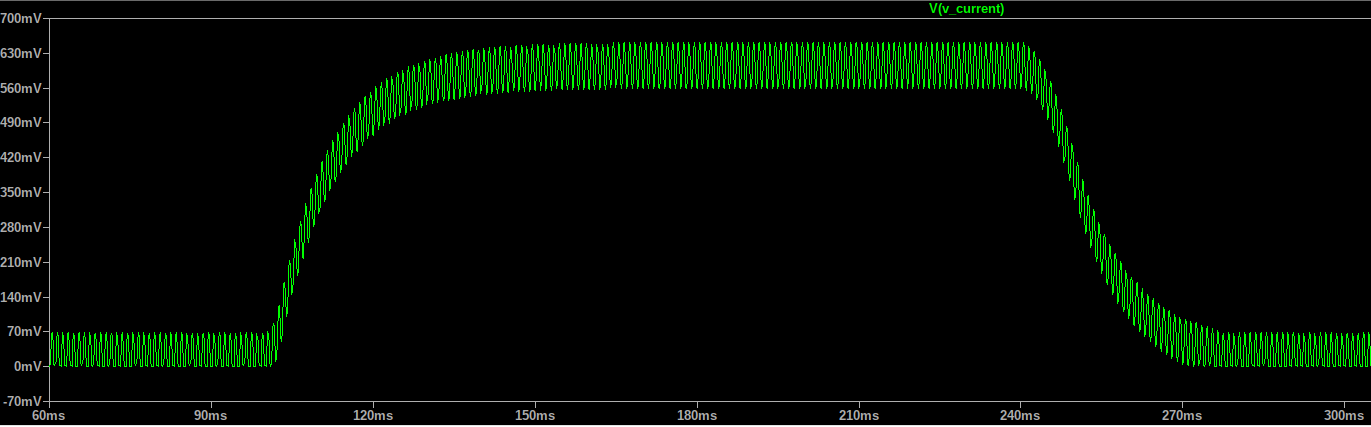
\includegraphics[width=.6\linewidth]{Figures/simulation_response}
   \captionof{figure}{Amplifier output in response to step input}
   \label{fig:simulation response}
\end{figure}

\begin{figure}[h!]
   \centering
   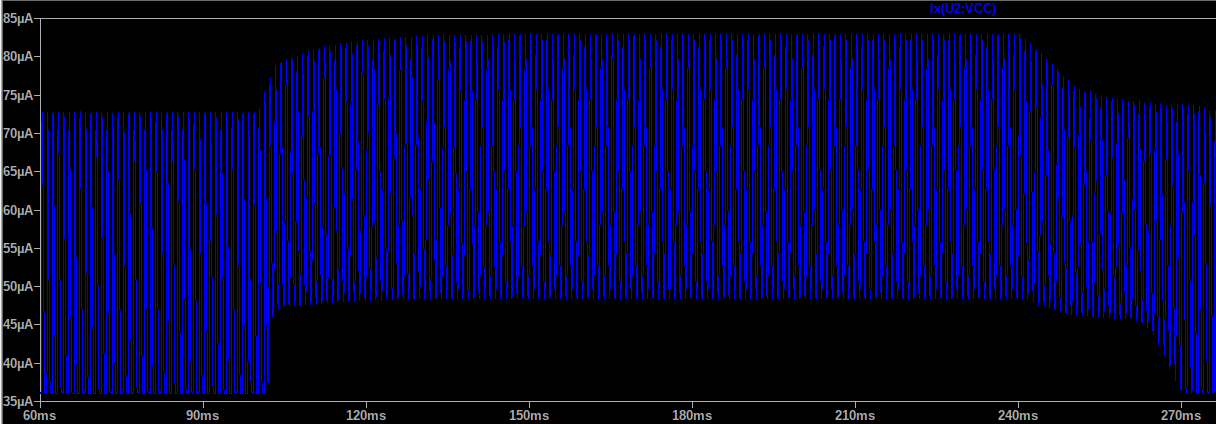
\includegraphics[width=.5\linewidth]{Figures/simulation_current}
   \captionof{figure}{Current draw of op-amp}
   \label{fig:simulation_current}
\end{figure}

As can be seen, all specifications were adhered to:
\begin{itemize}
   \item The noise level at idle is well below the 250 mV requirement.
   \item The step response input changes 20-25 ms, which is below the 100 ms requirement.
   \item The power draw of the circuit (as measure at the positive terminal of the op-amp) is less than 85 uA, which is much less than the specified 150 uA.
\end{itemize}

Lastly, the input simulation parameters were modified during testing to analyze the various output voltages for different input currents. For input currents of 400mA, 500mA, 800mA and 1A,
the output voltages were 1.22V, 1.52, 2.43 and 3.024 V respectively. This matches perfectly with the initial design.